% Copyright (c)  2005-2010 EDF-EADS-PHIMECA.
% Permission is granted to copy, distribute and/or modify this document
% under the terms of the GNU Free Documentation License, Version 1.2
% or any later version published by the Free Software Foundation;
% with no Invariant Sections, no Front-Cover Texts, and no Back-Cover
% Texts.  A copy of the license is included in the section entitled "GNU
% Free Documentation License".
\renewcommand{\filename}{docUC_InputNoData_Mixture.tex}
\renewcommand{\filetitle}{UC : Creation  of a nD distribution from a Mixture}

% \HeaderNNIILevel
% \HeaderIILevel
\HeaderIIILevel



\index{Distribution!Mixture}
\index{Graph!PDF-CDF curves}
\index{Graph Manipulation!Bounding box}
\index{Graph Manipulation!ViewImage}
\index{Graph Manipulation!Show}

In Open TURNS, a Mixture is a distribution which probability density function is a linear combination of probability density functions.\\

The objective of this Use Case is to model a distribution, defined as a mixture :
\begin {equation}\label{mixPDF}
  p(\vect{x}) = \sum_{i=1}^{n} a_i p_i(\vect{x})
\end{equation}
where 
\begin {equation}\label{mixcons}
\sum_{i=1}^{n} a_i = 1
\end{equation}
and 
\begin {equation}\label{mixcons2}
 \forall i,  \, a_i \geq 0
\end{equation}

Open TURNS automatically normalizes the  weights so the User can give $a_i$ which don't verify the constraint (\ref{mixcons}). \\
By default, the weights are taken equal to $\frac{1}{n}$.\\

Details on each object may be found in the User Manual  (\href{OpenTURNS_UserManual_TUI.pdf}{see User Manual - Distributions / Linear combination of probability density functions}).\\

The example here is a mixture of three 1D distributions Triangular(1.0, 2.0, 4.0), Normal(-1.0, 1.0) and Uniform(5.0, 6.0), with respective weights : (0.2, 0.3, 0.5).\\
The PDF and CDF graphs the mixture distribution are drawn in Figures \ref{mixtureGraphPDF} and  \ref{mixtureGraphCDF}.

\textspace\\
\noindent%
\requirements{
  \begin{description}
  \item[$\bullet$] none
  \end{description}
}
{
  \begin{description}
  \item[$\bullet$] a mixture distribution : {\itshape myMixture}
  \item[type:] Mixture
  \item[$\bullet$] a random input vector : {\itshape input}
  \item[type:] RandomVector which implementation is a UsualRandomVector
  \end{description}
}

\textspace\\
Python script for this UseCase :

\begin{lstlisting}

  # Create the three distributions and affect them their relative weights 

  # Triangular(1.0, 2.0, 4.0)
  triang = Triangular(1.0, 2.0, 4.0)
  triang.setWeight(20)

  # Normal(-1.0, 1.0)
  norm = Normal(-1.0, 1.0)
  norm.setWeight(50)

  # Uniform(5.0, 6.0)
  unif = Uniform(5.0,6.0)
  unif.setWeight(30)

  # Create a collection of distribution
  aCollection = DistributionCollection( (triang, norm, unif) )

  # Instanciate one distribution object
  myMixture = Mixture(aCollection)

  # Alternate definition of the weights
  myWeights = [0.20, 0.50, 0.30]
  myMixture = Mixture(aCollection, myWeights)

  # Alternate definition of the weights, not normalized
  myWeights = [2.0, 5.0, 3.0]
# The normalization is done automatically
  myMixture = Mixture(aCollection, myWeights)

  # Draw the PDF and CDF of this distribution
  # Impose a x-range
  myMixture_pdf = myMixture.drawPDF(-3.0,7.0)
  myMixture_pdf.setLegendPosition("topleft")

  myMixture_cdf = myMixture.drawCDF(-3.0,7.0)

  # Or impose a bounding box : x-range and y-range
  # boundingBox = [xmin, xmax, ymin, ymax]
  myBoundingBox = NumericalPoint( (xmin, xmax, ymin, ymax) )
  myMixture_cdf.setBoundingBox(myBoundingBox)

  # In order to see the graphs without creating the files .EPS, .PNG, .PDF and .FIG
  Show(myMixture_pdf)
  Show(myMixture_cdf)

  # Create the files .EPS, .PNG, .PDF and .FIG
  myMixture_pdf.draw("pdf_Mixture")
  myMixture_cdf.draw("cdf_Mixture")

  # Visualize the file .PNG wihthin the TUI
  ViewImage(myMixture_pdf.getBitmap())
  ViewImage(myMixture_cdf.getBitmap())
\end{lstlisting}
\textspace\\


\begin{figure}[H]
  \begin{center}
    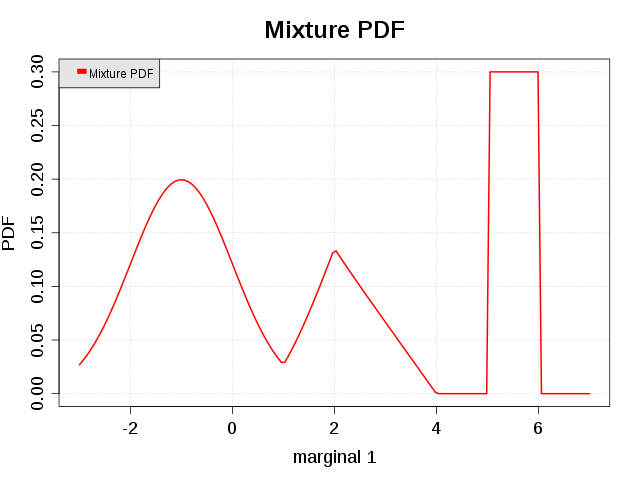
\includegraphics[width=10cm]{pdf_Mixture.png}
    \caption{PDF of the Mixture distribution = 0.2*Triangular(1.0, 2.0, 4.0) + 0.5*Normal(-1.0, 1.0) + 0.3*Uniform(5.0, 6.0)}
    \label{mixtureGraphPDF}
  \end{center}
\end{figure}

\begin{figure}[H]
  \begin{center}
    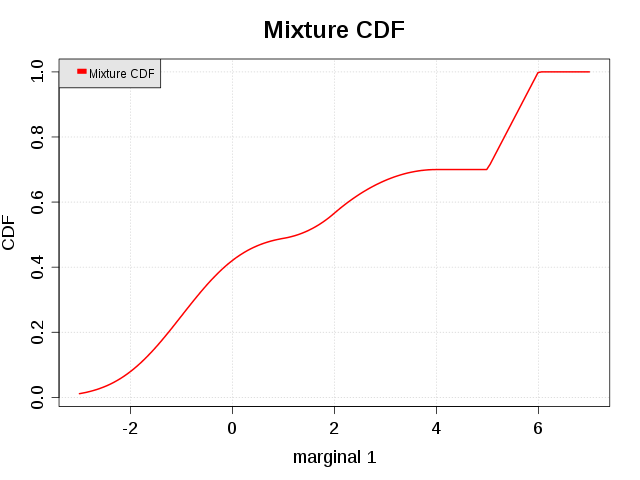
\includegraphics[width=10cm]{cdf_Mixture.png}
    \caption{CDF of the Mixture distribution = 0.2*Triangular(1.0, 2.0, 4.0) + 0.5*Normal(-1.0, 1.0) + 0.3*Uniform(5.0, 6.0)}
    \label{mixtureGraphCDF}
  \end{center}
\end{figure}

